\documentclass{standalone}
\usepackage{tikz}
\usetikzlibrary{patterns, positioning}
\usepackage[sfdefault]{ClearSans} %% option 'sfdefault' activates Clear Sans as the default text font
\usepackage[T1]{fontenc}

\begin{document}
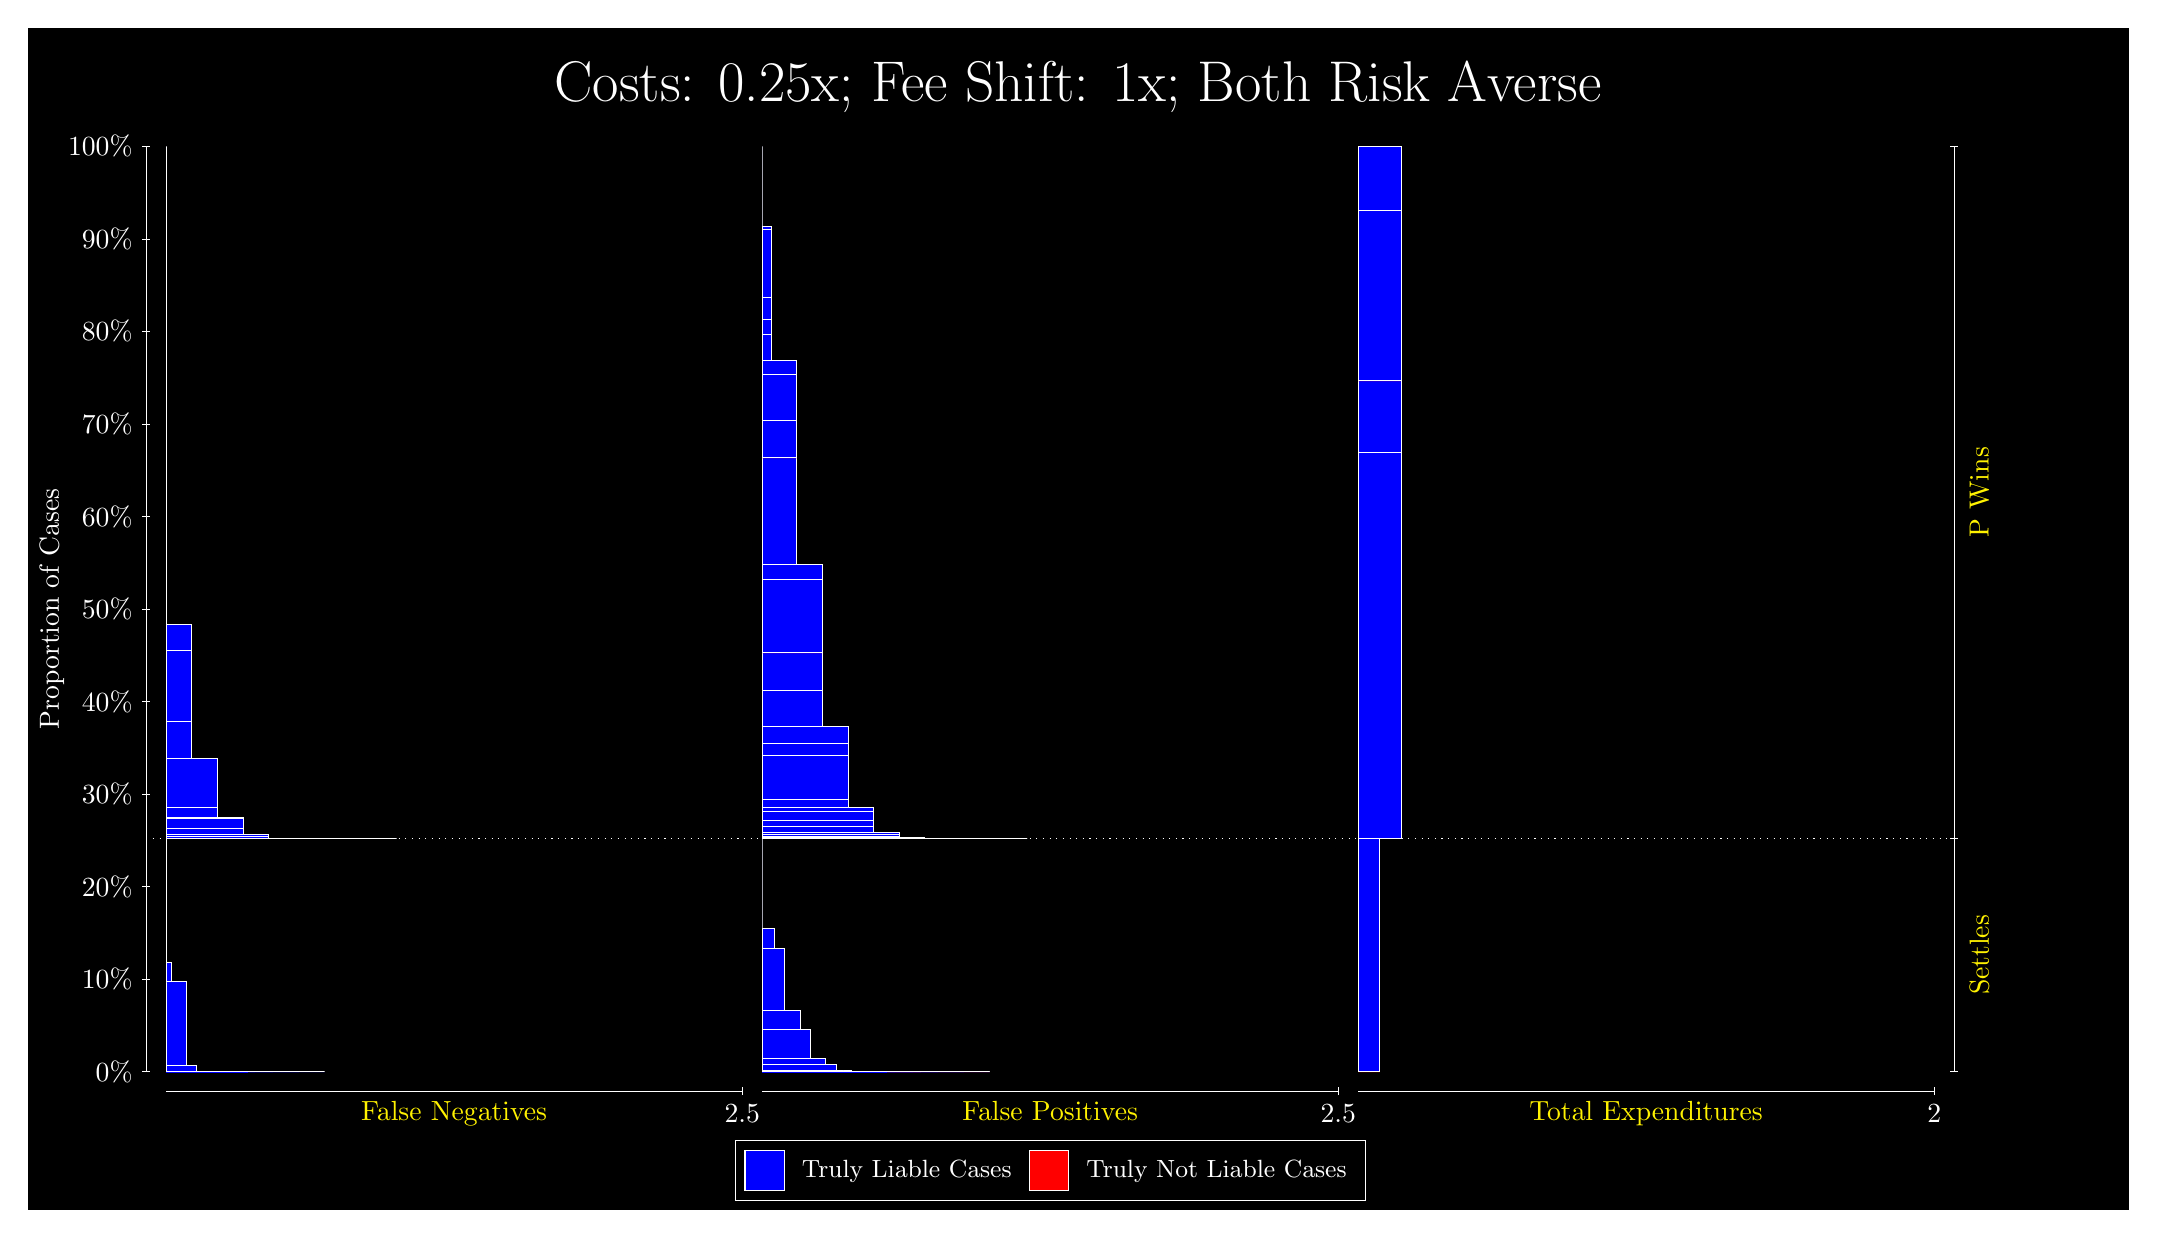
\begin{tikzpicture}
\draw[fill=black] (0,0) rectangle (26.667,15);
\draw[text=white] (0,13.5) rectangle (26.667,15) node[midway] {\huge Costs: 0.25x; Fee Shift: 1x; Both Risk Averse};
\draw[white, very thin] (1.5,1.75) -- (1.5,13.5);
\node[rotate=90, text=white, anchor=center] at (0.3, 7.625) {Proportion of Cases};
\draw[white, very thin] (1.45,1.75) -- (1.55,1.75);
\node[text=white, anchor=east] at (1.45, 1.75) {0\%};
\draw[white, very thin] (1.45,2.925) -- (1.55,2.925);
\node[text=white, anchor=east] at (1.45, 2.925) {10\%};
\draw[white, very thin] (1.45,4.1) -- (1.55,4.1);
\node[text=white, anchor=east] at (1.45, 4.1) {20\%};
\draw[white, very thin] (1.45,5.275) -- (1.55,5.275);
\node[text=white, anchor=east] at (1.45, 5.275) {30\%};
\draw[white, very thin] (1.45,6.45) -- (1.55,6.45);
\node[text=white, anchor=east] at (1.45, 6.45) {40\%};
\draw[white, very thin] (1.45,7.625) -- (1.55,7.625);
\node[text=white, anchor=east] at (1.45, 7.625) {50\%};
\draw[white, very thin] (1.45,8.8) -- (1.55,8.8);
\node[text=white, anchor=east] at (1.45, 8.8) {60\%};
\draw[white, very thin] (1.45,9.975) -- (1.55,9.975);
\node[text=white, anchor=east] at (1.45, 9.975) {70\%};
\draw[white, very thin] (1.45,11.15) -- (1.55,11.15);
\node[text=white, anchor=east] at (1.45, 11.15) {80\%};
\draw[white, very thin] (1.45,12.325) -- (1.55,12.325);
\node[text=white, anchor=east] at (1.45, 12.325) {90\%};
\draw[white, very thin] (1.45,13.5) -- (1.55,13.5);
\node[text=white, anchor=east] at (1.45, 13.5) {100\%};

\draw[white, very thin] (24.457,1.75) -- (24.457,13.5);
\draw[white, very thin] (24.407,1.75) -- (24.507,1.75);
\node[anchor=west] at (24.407, 1.75) {};
\draw[white, very thin] (24.407,4.7127) -- (24.507,4.7127);
\node[anchor=west] at (24.407, 4.7127) {};
\draw[white, very thin] (24.407,13.5) -- (24.507,13.5);
\node[anchor=west] at (24.407, 13.5) {};

\draw[white, very thin, fill=blue] (1.75,1.75) rectangle (3.7627,1.75);
\draw[white, very thin, fill=blue] (1.75,1.75) rectangle (3.4374,1.75);
\draw[white, very thin, fill=blue] (1.75,1.75) rectangle (3.1121,1.75);
\draw[white, very thin, fill=blue] (1.75,1.75) rectangle (2.8844,1.75);
\draw[white, very thin, fill=blue] (1.75,1.75) rectangle (2.7868,1.7503);
\draw[white, very thin, fill=blue] (1.75,1.7503) rectangle (2.5591,1.7503);
\draw[white, very thin, fill=blue] (1.75,1.7503) rectangle (2.4616,1.7575);
\draw[white, very thin, fill=blue] (1.75,1.7575) rectangle (2.2339,1.7575);
\draw[white, very thin, fill=blue] (1.75,1.7575) rectangle (2.1363,1.8307);
\draw[white, very thin, fill=blue] (1.75,1.8307) rectangle (2.0062,2.8922);
\draw[white, very thin, fill=blue] (1.75,2.8922) rectangle (1.9086,2.8922);
\draw[white, very thin, fill=blue] (1.75,2.8922) rectangle (1.811,3.1428);
\draw[white, very thin, fill=red] (1.75,3.1428) rectangle (1.75,3.1428);
\draw[white, very thin, fill=blue] (1.75,3.1428) rectangle (1.75,4.7127);
\draw[white, very thin, fill=blue] (1.75,4.7127) rectangle (4.6775,4.7127);
\draw[white, very thin, fill=blue] (1.75,4.7127) rectangle (4.3523,4.7127);
\draw[white, very thin, fill=blue] (1.75,4.7127) rectangle (4.027,4.7127);
\draw[white, very thin, fill=blue] (1.75,4.7127) rectangle (4.027,4.7127);
\draw[white, very thin, fill=blue] (1.75,4.7127) rectangle (3.7017,4.7128);
\draw[white, very thin, fill=blue] (1.75,4.7128) rectangle (3.7017,4.713);
\draw[white, very thin, fill=blue] (1.75,4.713) rectangle (3.3764,4.7176);
\draw[white, very thin, fill=blue] (1.75,4.7176) rectangle (3.0511,4.7347);
\draw[white, very thin, fill=blue] (1.75,4.7347) rectangle (3.0511,4.7589);
\draw[white, very thin, fill=blue] (1.75,4.7589) rectangle (2.7258,4.8424);
\draw[white, very thin, fill=blue] (1.75,4.8424) rectangle (2.7258,4.9618);
\draw[white, very thin, fill=blue] (1.75,4.9618) rectangle (2.7258,4.9794);
\draw[white, very thin, fill=blue] (1.75,4.9794) rectangle (2.4006,5.1082);
\draw[white, very thin, fill=blue] (1.75,5.1082) rectangle (2.4006,5.7306);
\draw[white, very thin, fill=blue] (1.75,5.7306) rectangle (2.0753,6.1945);
\draw[white, very thin, fill=blue] (1.75,6.1945) rectangle (2.0753,7.1031);
\draw[white, very thin, fill=blue] (1.75,7.1031) rectangle (2.0753,7.4338);
\draw[white, very thin, fill=red] (1.75,7.4338) rectangle (1.75,7.4338);
\draw[white, very thin, fill=blue] (1.75,7.4338) rectangle (1.75,13.5);
\draw[white, very thin, fill=red] (9.3189,1.75) rectangle (12.21,1.75);
\draw[white, very thin, fill=blue] (9.3189,1.75) rectangle (12.21,1.75);
\draw[white, very thin, fill=blue] (9.3189,1.75) rectangle (11.885,1.75);
\draw[white, very thin, fill=blue] (9.3189,1.75) rectangle (11.559,1.75);
\draw[white, very thin, fill=red] (9.3189,1.75) rectangle (11.332,1.75);
\draw[white, very thin, fill=blue] (9.3189,1.75) rectangle (11.332,1.75);
\draw[white, very thin, fill=blue] (9.3189,1.75) rectangle (11.234,1.75);
\draw[white, very thin, fill=blue] (9.3189,1.75) rectangle (11.006,1.75);
\draw[white, very thin, fill=blue] (9.3189,1.75) rectangle (10.909,1.7503);
\draw[white, very thin, fill=blue] (9.3189,1.7503) rectangle (10.681,1.7503);
\draw[white, very thin, fill=blue] (9.3189,1.7503) rectangle (10.583,1.7575);
\draw[white, very thin, fill=red] (9.3189,1.7575) rectangle (10.453,1.7575);
\draw[white, very thin, fill=blue] (9.3189,1.7575) rectangle (10.453,1.768);
\draw[white, very thin, fill=blue] (9.3189,1.768) rectangle (10.356,1.768);
\draw[white, very thin, fill=blue] (9.3189,1.768) rectangle (10.258,1.8462);
\draw[white, very thin, fill=blue] (9.3189,1.8462) rectangle (10.128,1.9243);
\draw[white, very thin, fill=blue] (9.3189,1.9243) rectangle (10.03,1.9243);
\draw[white, very thin, fill=blue] (9.3189,1.9243) rectangle (9.9328,2.2818);
\draw[white, very thin, fill=blue] (9.3189,2.2818) rectangle (9.8027,2.5333);
\draw[white, very thin, fill=blue] (9.3189,2.5333) rectangle (9.7051,2.5333);
\draw[white, very thin, fill=blue] (9.3189,2.5333) rectangle (9.6076,3.3199);
\draw[white, very thin, fill=blue] (9.3189,3.3199) rectangle (9.4774,3.5705);
\draw[white, very thin, fill=blue] (9.3189,3.5705) rectangle (9.3799,3.5705);
\draw[white, very thin, fill=blue] (9.3189,3.5705) rectangle (9.3189,4.7127);
\draw[white, very thin, fill=red] (9.3189,4.7127) rectangle (12.686,4.7127);
\draw[white, very thin, fill=blue] (9.3189,4.7127) rectangle (12.686,4.7127);
\draw[white, very thin, fill=red] (9.3189,4.7127) rectangle (12.36,4.7127);
\draw[white, very thin, fill=blue] (9.3189,4.7127) rectangle (12.36,4.7127);
\draw[white, very thin, fill=red] (9.3189,4.7127) rectangle (12.035,4.7127);
\draw[white, very thin, fill=blue] (9.3189,4.7127) rectangle (12.035,4.7127);
\draw[white, very thin, fill=blue] (9.3189,4.7127) rectangle (12.035,4.7127);
\draw[white, very thin, fill=blue] (9.3189,4.7127) rectangle (12.035,4.7127);
\draw[white, very thin, fill=red] (9.3189,4.7127) rectangle (11.71,4.7127);
\draw[white, very thin, fill=blue] (9.3189,4.7127) rectangle (11.71,4.7132);
\draw[white, very thin, fill=blue] (9.3189,4.7132) rectangle (11.71,4.7133);
\draw[white, very thin, fill=red] (9.3189,4.7133) rectangle (11.384,4.7133);
\draw[white, very thin, fill=blue] (9.3189,4.7133) rectangle (11.384,4.7167);
\draw[white, very thin, fill=blue] (9.3189,4.7167) rectangle (11.384,4.7208);
\draw[white, very thin, fill=blue] (9.3189,4.7208) rectangle (11.059,4.7398);
\draw[white, very thin, fill=red] (9.3189,4.7398) rectangle (11.059,4.7398);
\draw[white, very thin, fill=blue] (9.3189,4.7398) rectangle (11.059,4.7636);
\draw[white, very thin, fill=blue] (9.3189,4.7636) rectangle (11.059,4.7828);
\draw[white, very thin, fill=blue] (9.3189,4.7828) rectangle (10.734,4.8615);
\draw[white, very thin, fill=blue] (9.3189,4.8615) rectangle (10.734,4.9465);
\draw[white, very thin, fill=red] (9.3189,4.9465) rectangle (10.734,4.9465);
\draw[white, very thin, fill=blue] (9.3189,4.9465) rectangle (10.734,5.0587);
\draw[white, very thin, fill=blue] (9.3189,5.0587) rectangle (10.734,5.1028);
\draw[white, very thin, fill=blue] (9.3189,5.1028) rectangle (10.409,5.2063);
\draw[white, very thin, fill=red] (9.3189,5.2063) rectangle (10.409,5.2063);
\draw[white, very thin, fill=blue] (9.3189,5.2063) rectangle (10.409,5.7697);
\draw[white, very thin, fill=blue] (9.3189,5.7697) rectangle (10.409,5.9143);
\draw[white, very thin, fill=blue] (9.3189,5.9143) rectangle (10.409,6.1322);
\draw[white, very thin, fill=blue] (9.3189,6.1322) rectangle (10.083,6.5982);
\draw[white, very thin, fill=blue] (9.3189,6.5982) rectangle (10.083,7.0697);
\draw[white, very thin, fill=red] (9.3189,7.0697) rectangle (10.083,7.0697);
\draw[white, very thin, fill=blue] (9.3189,7.0697) rectangle (10.083,8.0058);
\draw[white, very thin, fill=blue] (9.3189,8.0058) rectangle (10.083,8.1867);
\draw[white, very thin, fill=blue] (9.3189,8.1867) rectangle (9.758,9.5448);
\draw[white, very thin, fill=red] (9.3189,9.5448) rectangle (9.758,9.5448);
\draw[white, very thin, fill=blue] (9.3189,9.5448) rectangle (9.758,10.027);
\draw[white, very thin, fill=blue] (9.3189,10.027) rectangle (9.758,10.611);
\draw[white, very thin, fill=blue] (9.3189,10.611) rectangle (9.758,10.779);
\draw[white, very thin, fill=blue] (9.3189,10.779) rectangle (9.4327,11.11);
\draw[white, very thin, fill=blue] (9.3189,11.11) rectangle (9.4327,11.306);
\draw[white, very thin, fill=blue] (9.3189,11.306) rectangle (9.4327,11.581);
\draw[white, very thin, fill=blue] (9.3189,11.581) rectangle (9.4327,12.444);
\draw[white, very thin, fill=blue] (9.3189,12.444) rectangle (9.4327,12.482);
\draw[white, very thin, fill=blue] (9.3189,12.482) rectangle (9.3189,13.5);
\draw[white, very thin, fill=red] (16.888,1.75) rectangle (17.162,1.75);
\draw[white, very thin, fill=blue] (16.888,1.75) rectangle (17.162,4.7127);
\draw[white, very thin, fill=red] (16.888,4.7127) rectangle (17.437,4.7127);
\draw[white, very thin, fill=blue] (16.888,4.7127) rectangle (17.437,9.6142);
\draw[white, very thin, fill=red] (16.888,9.6142) rectangle (17.437,9.6142);
\draw[white, very thin, fill=blue] (16.888,9.6142) rectangle (17.437,10.525);
\draw[white, very thin, fill=red] (16.888,10.525) rectangle (17.437,10.525);
\draw[white, very thin, fill=blue] (16.888,10.525) rectangle (17.437,12.69);
\draw[white, very thin, fill=red] (16.888,12.69) rectangle (17.437,12.69);
\draw[white, very thin, fill=blue] (16.888,12.69) rectangle (17.437,13.5);
\draw[white, dotted] (1.5,4.7127) -- (24.457,4.7127);
\draw[white, very thin] (1.75,1.5) -- (9.0689,1.5);
\node[text=yellow, anchor=north] at (5.4094, 1.5) {False Negatives};
\draw[white, very thin] (9.0689,1.45) -- (9.0689,1.55);
\node[text=white, anchor=north] at (9.0689, 1.45) {2.5};

\draw[white, very thin] (9.3189,1.5) -- (16.638,1.5);
\node[text=yellow, anchor=north] at (12.978, 1.5) {False Positives};
\draw[white, very thin] (16.638,1.45) -- (16.638,1.55);
\node[text=white, anchor=north] at (16.638, 1.45) {2.5};

\draw[white, very thin] (16.888,1.5) -- (24.207,1.5);
\node[text=yellow, anchor=north] at (20.547, 1.5) {Total Expenditures};
\draw[white, very thin] (24.207,1.45) -- (24.207,1.55);
\node[text=white, anchor=north] at (24.207, 1.45) {2};

\node[text=yellow, centered, rotate=90] at (24.777, 3.2313) {Settles};
\node[text=yellow, centered, rotate=90] at (24.777, 9.1063) {P Wins};

\draw (12.978300999999998,1.5) node[draw=none] (baseCoordinate) {};
\begin{scope}[align=center]
        \matrix[scale=0.5, draw=white, below=0.5cm of baseCoordinate, nodes={draw}, column sep=0.1cm]{
            \node[rectangle, draw, minimum width=0.5cm, minimum height=0.5cm, fill=blue] {}; &
            \node[draw=none, font=\small, text=white] (B) {Truly Liable Cases}; &
            \node[rectangle, draw, minimum width=0.5cm, minimum height=0.5cm, fill=red] {}; &
            \node[draw=none, font=\small, text=white] (B) {Truly Not Liable Cases}; \\
            };
\end{scope}

\end{tikzpicture}
\end{document}